\documentclass{beamer}

\usetheme{Darmstadt}
\usefonttheme[onlylarge]{structurebold}
\setbeamerfont*{frametitle}{size=\normalsize,series=\bfseries}
\setbeamertemplate{navigation symbols}{}

% Standard packages

\usepackage[english]{babel}
\usepackage[latin1]{inputenc}
\usepackage{times}
\usepackage[T1]{fontenc}
\usepackage{float}
\usepackage{graphicx}
\usepackage{subcaption}
\usepackage{ifthen}
\usepackage{minted}
\usepackage{verbatim}
%\usepackage{multimedia}
\usepackage{movie15}

% Setup TikZ
\usepackage{tikz}
\usetikzlibrary{arrows}
\tikzstyle{block}=[draw opacity=0.7,line width=1.4cm]


% Author, Title, etc.
\title[Pure functional programming in Agent-Based Simulation] 
{%
  Pure functional programming \\ in Agent-Based Simulation
}

\author[Thaler]
{
  Jonathan~Thaler
}

\institute[University of Nottingham, Ningbo, China]
{
  University of Nottingham, Ningbo, China
}

\date[AIOP Seminar 2019]
{AIOP Seminar 2019}

% The main document
\begin{document}

\begin{frame}
  \titlepage
\end{frame}

\section{Introduction}
\begin{frame}{Research Questions}
\begin{itemize}
  \item \textbf{How} can we implement Agent-Based Simulation in (pure) functional programming using Haskell?
  \item \textbf{What} are the benefits and drawbacks?
\end{itemize}
\end{frame}

\begin{frame}{Hypotheses}
\begin{itemize}
  \item Arrive at deeper understanding of the computational aspects of ABS due to functional programmings focus on structure in computing. 
  \item Less bugs, more likely to be correct: stronger guarantees at compile time
  \item Better support for concurrency
  \item Natural fit for randomized property-based testing
  \item Step toward dependently typed ABS
\end{itemize}
\end{frame}

\section{Agent-Based Simulation}
\begin{frame}{Agent-Based Simulation (ABS)} 
  \begin{block}{Example}
    \textit{\textbf{Simulate} the spread of an infectious disease in a city. \\ What are the \textbf{dynamics} (peak, duration of disease)?}
  \end{block}
  
  \begin{enumerate}
    \item Start with population \, \, \, \, \, \, \, $\to$ Agents
 	\item Situated in City \, \, \, \, \, \, \, \, \, \, \, \,\, $\to$ Environment
 	\item Interacting with each other \, $\to$ Local interactions
 	\item Creating dynamics \, \, \, \, \, \, \, \,\,\, $\to$ Emergent system behaviour
 	\item Therefore ABS \, \, \, \, \, \, \, \, \, \, \, \,\,\, $\to$ Bottom-up approach
  \end{enumerate}
\end{frame}

\begin{frame}{SIR Model}
  
\includegraphics[width=0.7\textwidth]{./fig/SIR_transitions.png}
  
  \begin{itemize}
    \item Population size $N = 1,000$
 	\item Contact rate $\beta = 5$
 	\item Infection probability $\gamma = 0.05$
 	\item Illness duration $\delta = 15$
 	\item 1 initially infected agent
  \end{itemize}
    
  \begin{block}{System Dynamics}
    Top-Down, formalised using Differential Equations, give rise to dynamics.
  \end{block}
\end{frame}

\begin{frame}{SIR Model Dynamics}
  \center
  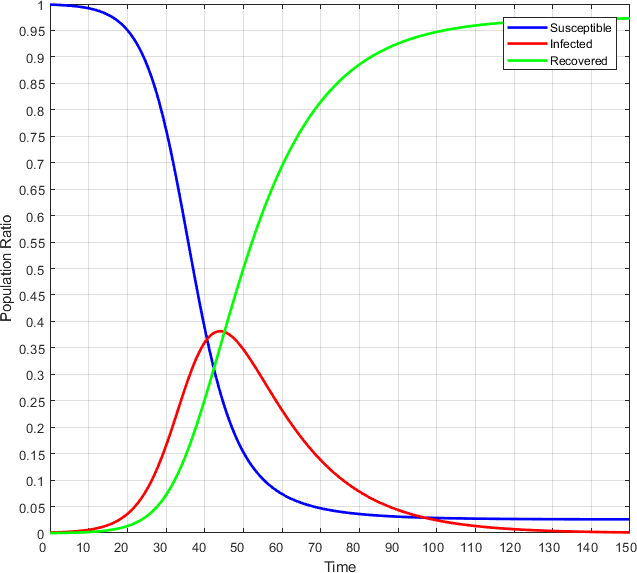
\includegraphics[width=0.7\textwidth]{./fig/SIR_SD_001dt.png}
\end{frame}

\begin{frame}[fragile]{Defining Spatiality}
\begin{figure}
\begin{center}

\includegraphics[width=0.2\textwidth]{./fig/moore.png}
\caption*{Moore Neighbourhood}
\end{center}
\end{figure}
\end{frame}

\begin{frame}{Spatial Dynamics}
\begin{figure}
\begin{center}
	\begin{tabular}{c c}
		\begin{subfigure}[b]{0.4\textwidth}
			\centering
			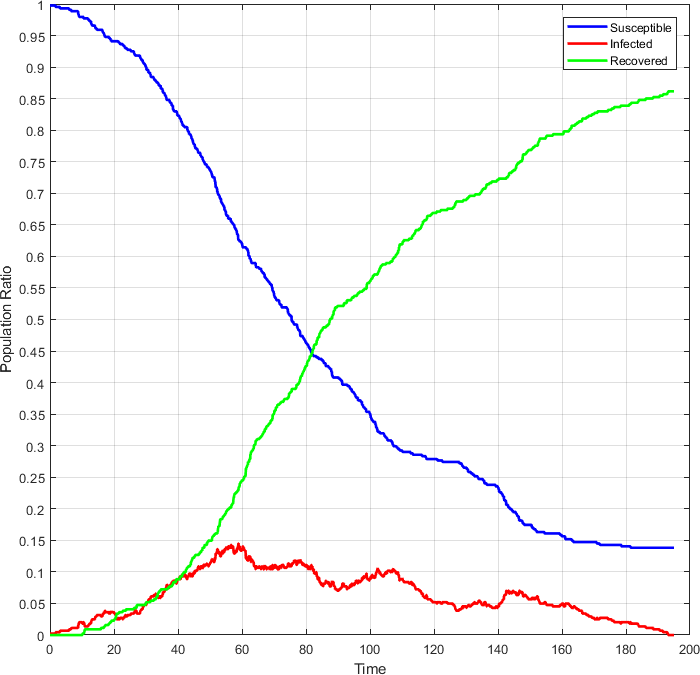
\includegraphics[width=0.95\textwidth, angle=0]{./fig/SIR_Dunai_dt001.png}
			\caption*{Agent-Based}
		\end{subfigure}
    	
    	&
  
		\begin{subfigure}[b]{0.4\textwidth}
			\centering
			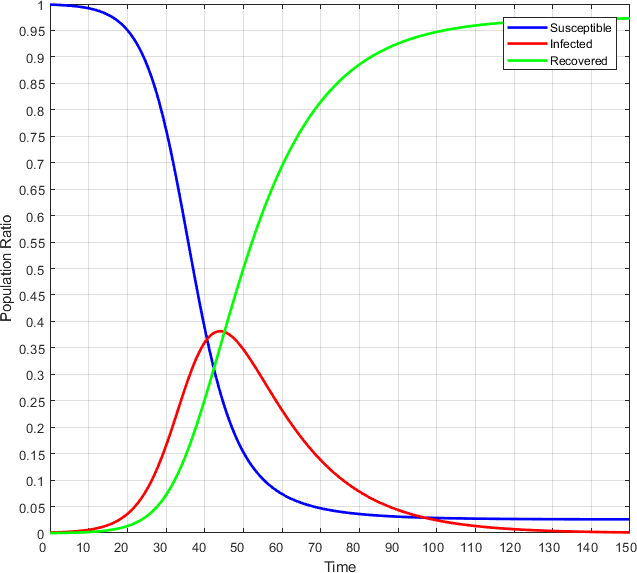
\includegraphics[width=1\textwidth, angle=0]{./fig/SIR_SD_001dt.png}
			\caption*{System Dynamics}
		\end{subfigure}
	\end{tabular}
\end{center}
\end{figure}
\end{frame}

\begin{frame}{Spatial Visualisation}
%\movie[width=10cm,height=5.5cm]{Dynamics 21x21 2D Environment}{./video/SIR_DUNAI_dt001.mp4}
\includemovie[rate=2]{11cm}{6.5cm}{./video/SIR_DUNAI_dt001.mp4}
\end{frame}

\section{Pure functional programming}
TODO: explain monads: declare type of side-effects statically at compile-time

\section{Implementing pure functional ABS}
\begin{frame}{How to implement ABS?}
  \begin{block}{Established, state-of-the-art approach in ABS}
	Object-Oriented Programming in Python, Java,...
  \end{block}
  
  \begin{block}{We want (pure) functional programming}
	Purity, explicit about side-effects, declarative, reasoning, parallelism, concurrency, property-based testing,...
  \end{block}
  
  \begin{block}{How can we do it?}
  	Functional Reactive Programming
  \end{block}
\end{frame}

\begin{frame}{Arrowized Functional Reactive Programming (AFRP)}
  \begin{itemize}
    \item Continuous- \& discrete-time systems in FP
 	\item Signal Function 
 	\item Events
 	\item Effects like random-numbers, global state, concurrency
 	%\item Running signal-functions in pure way
 	\item \textit{Arrowized} FRP using the \textit{Dunai} library
  \end{itemize}
\end{frame}

\begin{frame}{Monadic Stream Functions (MSF)}
  \begin{block}{Process over time}
  \begin{flalign*}
	SF \, \alpha \, \beta \approx Signal \, \alpha \rightarrow Signal \, \beta \\
	Signal \, \alpha \approx Time \rightarrow \alpha 
  \end{flalign*}
  \end{block}
  
  \begin{block}{Agents as Signal Functions}
  \begin{itemize}
  	\item Clean interface (input / output)
  	\item Pro-activity by perceiving time
  \end{itemize}
  \end{block}
\end{frame}

\begin{frame}[fragile]{FRP combinators}
\begin{block}{Dynamic change of behaviour}
\begin{minted}[fontsize=\footnotesize]{haskell}
switch :: SF inp (out, Event e) 
       -> (e -> SF inp out) 
       -> SF inp out
\end{minted}
\end{block}

\begin{block}{Stochastic event source}
\begin{minted}[fontsize=\footnotesize]{haskell}
occasionally :: RandomGen g  
             => g -> Time -> b -> SF a (Event b)
\end{minted}
\end{block}

\begin{block}{Random number stream}
\begin{minted}[fontsize=\footnotesize]{haskell}
noiseR :: (RandomGen g, Random b) 
       => (b, b) -> g -> SF a b
\end{minted}
\end{block}

\begin{block}{Infinitesimal delay (1 step)}
\begin{minted}[fontsize=\footnotesize]{haskell}
iPre :: a -> SF a a
\end{minted}
\end{block}
\end{frame}


\section{Conclusion}

\begin{frame}{Conclusion}
  \begin{itemize}
    \item Purity guarantees reproducibility 
    \item Enforce and guarantee update semantics 
    \item Performance low but STM improves a lot
    \item Property-based testing is a perfect match!
    \item Further research: dependent types
  \end{itemize}
\end{frame}

\begin{frame}{}
  \begin{center}
  Thank You!
  \end{center}
\end{frame}
\end{document}